% \chapter{État de l'art}
% \label{chap:2}

% La détection et la reconnaissance de véhicules militaires sont des domaines de recherche essentiels en intelligence artificielle, en particulier dans le contexte de la défense. Avec l'évolution rapide des technologies de deep learning, plusieurs études ont exploré et développé des modèles visant à améliorer la précision et la robustesse de ces systèmes. Cet état de l'art analyse les articles pertinents sur le sujet, compare les approches existantes et identifie les principaux défis techniques associés à la détection de véhicules militaires.

% \section{Articles étudiés}

% Plusieurs articles ont été examinés pour comprendre les différentes approches de détection de véhicules militaires. Parmi eux, trois publications se distinguent par la qualité et la pertinence de leurs contributions :

% \begin{itemize}
%     \item Kamran et al. (2020) \cite{kamran2020}, qui explore l'utilisation de réseaux de neurones convolutifs pour la détection automatisée de véhicules militaires à partir d'images aériennes.
%     \item Gupta et al. (2021) \cite{gupta2021}, qui examine l'application de techniques de deep learning pour la détection de véhicules dans des images aériennes, en mettant un accent particulier sur l'amélioration des modèles existants.
%     \item Dijk et al. (2020) \cite{spie2020}, qui se concentre sur la détection longue distance de personnes et de véhicules, en analysant les performances de différents modèles de deep learning.
% \end{itemize}

% Ces articles fournissent une base solide pour comparer les différentes approches et comprendre les enjeux techniques de la détection de véhicules militaires.

% \section{Technologies de Détection d'Objets dans les Images Aériennes}

% La détection d'objets dans les images aériennes a évolué rapidement avec l'avènement des techniques de deep learning. Traditionnellement, les méthodes de détection reposaient sur des techniques de traitement d'image basées sur des caractéristiques définies manuellement, telles que les transformées de Hough, les descripteurs de contours et les filtres de Sobel. Cependant, ces méthodes ont montré des limites importantes en termes de précision et de robustesse, particulièrement dans des environnements complexes où les objets peuvent varier en taille, orientation et conditions d'éclairage.

% Avec l'émergence des \textbf{réseaux de neurones convolutifs} (CNN), une nouvelle ère a commencé pour la détection d'objets. Les modèles CNN, tels que YOLO (You Only Look Once), SSD (Single Shot MultiBox Detector), et Faster R-CNN, ont permis de franchir un cap en matière de précision et d'efficacité, en apprenant directement des données d'entraînement pour extraire des caractéristiques complexes adaptées aux spécificités des objets présents dans les images aériennes \cite{kamran2020}.

% Cependant, l'application de ces modèles aux images aériennes, et plus particulièrement à la détection de véhicules militaires, présente des défis uniques. Les véhicules sont souvent de petite taille, peuvent être camouflés, et sont situés dans des environnements visuellement encombrés. Ces facteurs compliquent la tâche des algorithmes de détection classiques, nécessitant des ajustements spécifiques dans les architectures de réseaux neuronaux et les techniques de prétraitement des données \cite{gupta2021}.

% \section{Détection de Véhicules Militaires}

% \subsection{Enjeux et Défis Spécifiques}

% La détection de véhicules militaires dans les images aériennes pose des défis particuliers qui ne sont pas rencontrés dans la détection de véhicules civils. Ces défis incluent le camouflage actif, la dissimulation dans des environnements naturels complexes, et la variabilité des configurations de véhicules militaires. Contrairement aux véhicules civils, les véhicules militaires peuvent varier considérablement en termes de taille, de forme, et de coloration, ce qui complique davantage leur détection \cite{kamran2020}.

% En outre, les véhicules militaires sont souvent capturés dans des conditions difficiles, telles que des angles de vue inhabituels (ex. la Figure~\ref{fig:comparaison_vehicles} des images aériennes prises à basse altitude), des environnements à faible luminosité, ou des contextes où les véhicules sont partiellement cachés ou occultés par d'autres objets. Ces scénarios augmentent la difficulté de la détection, nécessitant des algorithmes capables de gérer ces complexités.

% \begin{figure}[H]
%     \centering
%     \begin{subfigure}[b]{0.45\textwidth}
%         \centering
%         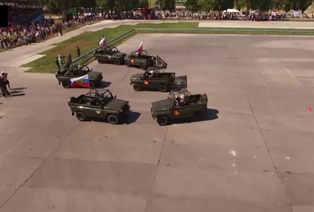
\includegraphics[width=\textwidth]{./images/military-vehicul.png}
%         \caption{Véhicules militaires}
%         \label{fig:military-vehicles}
%     \end{subfigure}
%     \hfill
%     \begin{subfigure}[b]{0.45\textwidth}
%         \centering
%         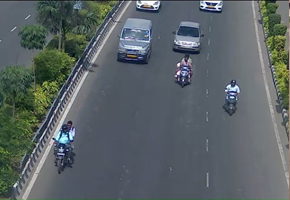
\includegraphics[width=\textwidth]{./images/non-military-vehicul.png}
%         \caption{Véhicules non militaires}
%         \label{fig:non-military-vehicles}
%     \end{subfigure}
%     \caption{Images aériennes à basse altitude de véhicules réels \cite[p.~2]{kamran2020}.}
%     \label{fig:comparaison_vehicles}
% \end{figure}

% \subsection{Approches Modernes pour la Détection des Véhicules Militaires}

% Les approches modernes pour la détection des véhicules militaires utilisent principalement des techniques de deep learning, avec un accent sur les réseaux de neurones convolutifs (CNN). Trois architectures principales sont souvent utilisées pour cette tâche : \textbf{Faster R-CNN}, \textbf{R-FCN} (Region-based Fully Convolutional Networks), et \textbf{SSD} (Single Shot MultiBox Detector). Ces architectures ont montré leur efficacité pour détecter et classifier les véhicules militaires, même dans des environnements complexes et encombrés \cite{kamran2020}.

% Parmi ces architectures, Faster R-CNN a démontré une supériorité dans plusieurs études en raison de sa capacité à générer rapidement des propositions de régions et à classifier les objets avec une grande précision. Cependant, pour des véhicules de petite taille ou dans des contextes de faible contraste, des ajustements spécifiques des hyperparamètres et des techniques de data augmentation sont souvent nécessaires pour améliorer les performances des modèles \cite{gupta2021}.

% L'utilisation de \textbf{datasets spécialisés} est également importante. Par exemple, Kamran et al. \cite{kamran2020} ont développé un dataset spécifique pour la détection de véhicules militaires à partir d'images aériennes prises à basse altitude. Ce dataset combine des images réelles et des images synthétiques, permettant ainsi de pallier le manque de données réelles disponibles pour l'entraînement des modèles.

% Enfin, les techniques de \textbf{génération de données synthétiques}, comme celles basées sur les GANs (Generative Adversarial Networks), sont de plus en plus utilisées pour enrichir les datasets et améliorer la robustesse des modèles de détection face à la variabilité des conditions d'acquisition des images \cite{spie2020}.

% \section{Étude Comparative des Approches}

% \subsection{Valeur des Modèles}

% Les articles analysés mettent en évidence l'efficacité des modèles de deep learning, en particulier des réseaux de neurones convolutifs (CNN), dans la détection de véhicules militaires. Les études de Kamran et al. \cite{kamran2020} et de Gupta et al. \cite{gupta2021} démontrent que les modèles comme YOLO et Faster R-CNN surpassent largement les méthodes traditionnelles en termes de précision et de rapidité de détection.

% Cependant, une comparaison plus détaillée révèle que chaque modèle a ses avantages et ses limitations. Par exemple, \textbf{YOLO} est rapide et adapté aux applications en temps réel, mais peut manquer de précision pour les objets de petite taille ou en partie occultés. À l'inverse, \textbf{Faster R-CNN} offre une meilleure précision, mais au prix d'une complexité computationnelle accrue, ce qui le rend moins adapté aux environnements où les ressources sont limitées.

% \subsection{Qualité des Données et Entraînement des Modèles}

% L'efficacité des modèles de deep learning dépend fortement de la qualité et de la quantité des données utilisées pour leur entraînement. Kamran et al. \cite{kamran2020} soulignent l'importance de disposer de datasets spécialisés, comprenant à la fois des images réelles et synthétiques, pour pallier le manque de données disponibles. Dans le même temps, Gupta et al. \cite{gupta2021} montrent que l'utilisation de techniques de data augmentation est importante pour améliorer la robustesse des modèles face aux variations des conditions d'acquisition des images.

% La génération de données synthétiques, notamment via des GANs, est également discutée comme une solution viable pour enrichir les datasets et permettre aux modèles de mieux généraliser. Cependant, cette approche introduit de nouveaux défis, notamment en termes de validation des modèles sur des données réelles.


% \subsection{Modèles Utilisés et Performances}

% Les performances des différents modèles sont évaluées en fonction de critères tels que la précision de la détection, le taux de faux positifs, et la robustesse face aux variations d'éclairage et de perspective. L'étude de Dijk et al. \cite{spie2020} compare les performances de plusieurs modèles sur des images à longue distance, montrant que les modèles comme \textbf{R-FCN} peuvent offrir un bon compromis entre précision et vitesse dans des environnements complexes.

% Néanmoins, la comparaison entre les modèles met également en lumière le besoin d'optimiser les hyperparamètres pour chaque contexte spécifique. Par exemple, l'ajustement des seuils de détection et l'utilisation de techniques de régularisation sont souvent nécessaires pour améliorer les performances dans des conditions de faible visibilité.
% \begin{table}[H]
%     \centering
%     \begin{tabularx}{\textwidth}{|p{3.1cm}|p{2.1cm}|p{1.1cm}|p{2.2cm}|X|c|}
%         \hline
%         \textbf{Étude}                  & \textbf{Modèle} & \textbf{mAP (\%)} & \textbf{Temps d'inférence (ms)} & \textbf{Données}                       & \textbf{Classes} \\ \hline
%         Kamran et al. \cite{kamran2020} & Faster R-CNN    & 78                & 220                             & 5 000 images (réelles et synthétiques) & 3                \\ \hline
%         Kamran et al. \cite{kamran2020} & SSD             & 72                & 165                             & 5 000 images (réelles et synthétiques) & 3                \\ \hline
%         Gupta et al. \cite{gupta2021}   & YOLOv3          & 82                & 180                             & 6 742 images (réelles)                 & 5                \\ \hline
%         Gupta et al. \cite{gupta2021}   & SSD             & 75                & 160                             & 6 742 images (réelles)                 & 5                \\ \hline
%         Dijk et al. \cite{spie2020}     & CNN             & 55                & 250                             & 9 000 images (réelles)                 & 7                \\ \hline
%     \end{tabularx}
%     \caption{Comparaison des performances des modèles}
%     \label{tab:comparaison}
% \end{table}


% \subsection{Paramètres de Configuration des Modèles}

% Les performances des modèles de deep learning dépendent fortement des paramètres de configuration utilisés pendant l'entraînement. Dans cette section, nous comparons les principaux paramètres de configuration pour les modèles étudiés dans les différents articles.

% \begin{table}[H]
%     \centering
%     \begin{tabularx}{\textwidth}{|p{3cm}|p{2cm}|p{2cm}|p{2cm}|p{3cm}|p{2cm}|}
%         \hline
%         \textbf{Étude}                  & \textbf{Modèle} & \textbf{Taux d'apprentissage} & \textbf{Taille du batch} & \textbf{Nombre d'époques} & \textbf{Taille d'image (px)} \\ \hline
%         Kamran et al. \cite{kamran2020} & Faster R-CNN    & 0.001                         & 16                       & 50                        & 600x600                      \\ \hline
%         Kamran et al. \cite{kamran2020} & SSD             & 0.002                         & 32                       & 100                       & 300x300                      \\ \hline
%         Gupta et al. \cite{gupta2021}   & YOLOv3          & 0.0001                        & 32                       & 70                        & 416x416                      \\ \hline
%         Gupta et al. \cite{gupta2021}   & SSD             & 0.002                         & 24                       & 100                       & 300x300                      \\ \hline
%         Dijk et al. \cite{spie2020}     & CNN             & 0.0005                        & 24                       & 80                        & 512x512                      \\ \hline
%     \end{tabularx}
%     \caption{Comparaison des paramètres de configuration des modèles}
%     \label{tab:parametres}
% \end{table}

% Les paramètres de configuration ci-dessus montrent les choix effectués par les auteurs pour optimiser les performances des modèles dans des contextes spécifiques. Par exemple, la taille du batch et le taux d'apprentissage sont important pour la stabilité et la convergence du modèle. Dans l'étude de Kamran et al., un taux d'apprentissage plus élevé a été utilisé pour SSD, ce qui a permis d'accélérer l'entraînement, bien que cela puisse parfois mener à une instabilité si non contrôlé par un ajustement fin des hyperparamètres. En revanche, Gupta et al. ont opté pour un taux d'apprentissage plus faible pour YOLOv3, privilégiant une convergence plus lente mais plus stable, ce qui est souvent nécessaire pour des architectures complexes comme YOLOv3.

% Cette comparaison met en évidence l'importance d'ajuster les paramètres en fonction des spécificités du modèle et du contexte opérationnel, afin de maximiser les performances tout en minimisant les risques d'overfitting ou de sous-apprentissage.



% \section{Synthèse}

% L'analyse des articles révèle plusieurs défis techniques associés à la détection de véhicules militaires. Parmi eux, la gestion des données limitées et leur qualité, l'optimisation des modèles pour des environnements variés, et la réduction des biais introduits par les datasets sont les plus critiques.

% Un point clé soulevé par les études est la nécessité d'une approche équilibrée entre précision et efficacité computationnelle. Bien que des modèles plus complexes comme \textit{YOLOv3} offrent des performances supérieures, leur application en temps réel dans des environnements militaires reste limitée par les ressources disponibles. Par conséquent, des compromis sont souvent nécessaires en fonction des exigences spécifiques de la mission.

% Les défis spécifiques de la détection de véhicules militaires nécessitent l'utilisation de techniques avancées de deep learning et de datasets spécialisés. Les progrès récents dans ce domaine, combinés à l'utilisation de données synthétiques et de méthodes de data augmentation, offrent des perspectives prometteuses pour améliorer la précision et la robustesse des systèmes de détection dans des contextes militaires complexes.






































\chapter{État de l'art}
\label{chap:2}

La détection et la reconnaissance de véhicules militaires sont des domaines de recherche essentiels en intelligence artificielle, en particulier dans le contexte de la défense. Avec l'évolution rapide des technologies de deep learning, plusieurs études ont exploré et développé des modèles visant à améliorer la précision et la robustesse de ces systèmes. Cet état de l'art analyse les articles pertinents sur le sujet, compare les approches existantes et identifie les principaux défis techniques associés à la détection de véhicules militaires.

\section{Articles étudiés}

Plusieurs articles ont été examinés pour comprendre les différentes approches de détection de véhicules militaires. Parmi eux, trois publications se distinguent par la qualité et la pertinence de leurs contributions :

\begin{itemize}
    \item Kamran et al. (2020) \cite{kamran2020}, qui explore l'utilisation de réseaux de neurones convolutifs pour la détection automatisée de véhicules militaires à partir d'images aériennes.
    \item Gupta et al. (2021) \cite{gupta2021}, qui examine l'application de techniques de deep learning pour la détection de véhicules dans des images aériennes, en mettant un accent particulier sur l'amélioration des modèles existants.
    \item Dijk et al. (2020) \cite{spie2020}, qui se concentre sur la détection longue distance de personnes et de véhicules, en analysant les performances de différents modèles de deep learning.
\end{itemize}

Ces articles fournissent une base solide pour comparer les différentes approches et comprendre les enjeux techniques de la détection de véhicules militaires.



\section{Technologies de Détection d'Objets dans les Images}

La détection d'objets dans les images a évolué rapidement avec l'avènement des techniques de deep learning. Traditionnellement, les méthodes de détection reposaient sur des techniques de traitement d'image basées sur des caractéristiques définies manuellement, telles que les transformées de Hough, les descripteurs de contours et les filtres de Sobel. Cependant, ces méthodes ont montré des limites importantes en termes de précision et de robustesse, particulièrement dans des environnements complexes où les objets peuvent varier en taille, orientation et conditions d'éclairage.

Avec l'émergence des \textbf{réseaux de neurones convolutifs} (CNN), une nouvelle ère a commencé pour la détection d'objets (Figure~\ref{fig:inptu-Output-image}). Les modèles CNN, tels que YOLO (You Only Look Once), SSD (Single Shot MultiBox Detector), et Faster R-CNN, ont permis de franchir un cap en matière de précision et d'efficacité, en apprenant directement des données d'entraînement pour extraire des caractéristiques complexes adaptées aux spécificités des objets présents dans les images \cite{kamran2020, gupta2021}.

\begin{figure}[H]
    \centering
    \begin{subfigure}[b]{0.45\textwidth}
        \centering
        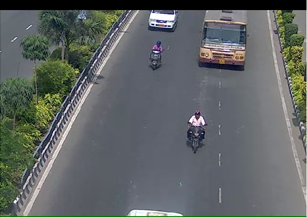
\includegraphics[width=\textwidth]{./images/input-image.png}
        \caption{Image d'entrée : contenant des véhicules}
    \end{subfigure}
    \hfill
    \begin{subfigure}[b]{0.45\textwidth}
        \centering
        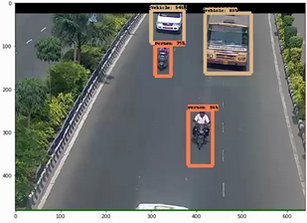
\includegraphics[width=\textwidth]{./images/output-image.png}
        \caption{Image de sortie : Reconnaissance des véhicules}
    \end{subfigure}
    \caption{Images aériennes à basse altitude de véhicules réels \cite[p.~3]{kamran2020}.}
    \label{fig:inptu-Output-image}
\end{figure}

\textbf{YOLOv3} \cite{redmon2016yolo} est particulièrement notable pour sa rapidité et son efficacité dans les applications en temps réel. Contrairement à d'autres modèles, YOLOv3 divise l'image en une grille et prédit simultanément plusieurs boîtes englobantes et leurs probabilités de classe, ce qui le rend extrêmement rapide. Cependant, cette rapidité se fait parfois au détriment de la précision, surtout pour les objets de petite taille ou partiellement occultés. Néanmoins, YOLOv3 reste un choix privilégié pour les applications nécessitant une détection rapide avec une précision acceptable, que ce soit pour des images capturées à partir d'une caméra embarquée, de vidéosurveillance, ou de systèmes aéroportés \cite{gupta2021}.

\textbf{SSD (Single Shot MultiBox Detector)} \cite{liu2016ssd} offre également une approche rapide mais légèrement plus précise que YOLO pour les objets de taille moyenne à grande. SSD divise l'image en plusieurs couches de caractéristiques, chacune spécialisée dans la détection d'objets de différentes tailles, ce qui améliore la précision tout en conservant une bonne vitesse d'inférence. Ce modèle est adapté à une grande variété d'applications, qu'il s'agisse de la surveillance vidéo, de la détection de véhicules dans des environnements urbains, ou de l'analyse d'images capturées par des drones \cite{kamran2020}.

Enfin, \textbf{Faster R-CNN} \cite{girshick2016rcnn} se distingue par sa précision supérieure, en particulier dans des environnements complexes où les objets sont petits ou partiellement cachés. Ce modèle utilise un réseau de propositions de région pour identifier les zones d'intérêt avant d'appliquer la classification, ce qui permet une détection plus précise. Cependant, cette approche est plus gourmande en ressources computationnelles et est moins adaptée aux environnements où les temps de réponse doivent être courts, comme dans les applications en temps réel nécessitant une haute précision \cite{kamran2020}.

L'application de ces modèles aux images, qu'elles soient issues de drones, de caméras de surveillance ou d'autres sources, présente des défis uniques. Les objets détectés peuvent être de petite taille, camouflés ou situés dans des environnements visuellement encombrés. Ces facteurs compliquent la tâche des algorithmes de détection classiques, nécessitant des ajustements spécifiques dans les architectures de réseaux neuronaux et les techniques de prétraitement des données \cite{gupta2021}.

De plus, l'utilisation de \textbf{datasets spécialisés} est cruciale pour entraîner ces modèles à détecter des objets dans des contextes variés. Par exemple, Kamran et al. \cite{kamran2020} ont développé un dataset spécifique pour la détection de véhicules militaires, combinant des images réelles et synthétiques, ce qui permet de pallier le manque de données réelles disponibles pour l'entraînement des modèles.

Enfin, les techniques de \textbf{génération de données synthétiques}, comme celles basées sur les GANs (Generative Adversarial Networks), sont de plus en plus utilisées pour enrichir les datasets et améliorer la robustesse des modèles de détection face à la variabilité des conditions d'acquisition des images, qu'il s'agisse d'images de terrain, aériennes ou issues de caméras fixes \cite{spie2020}.

\begin{figure}[H]
    \center
    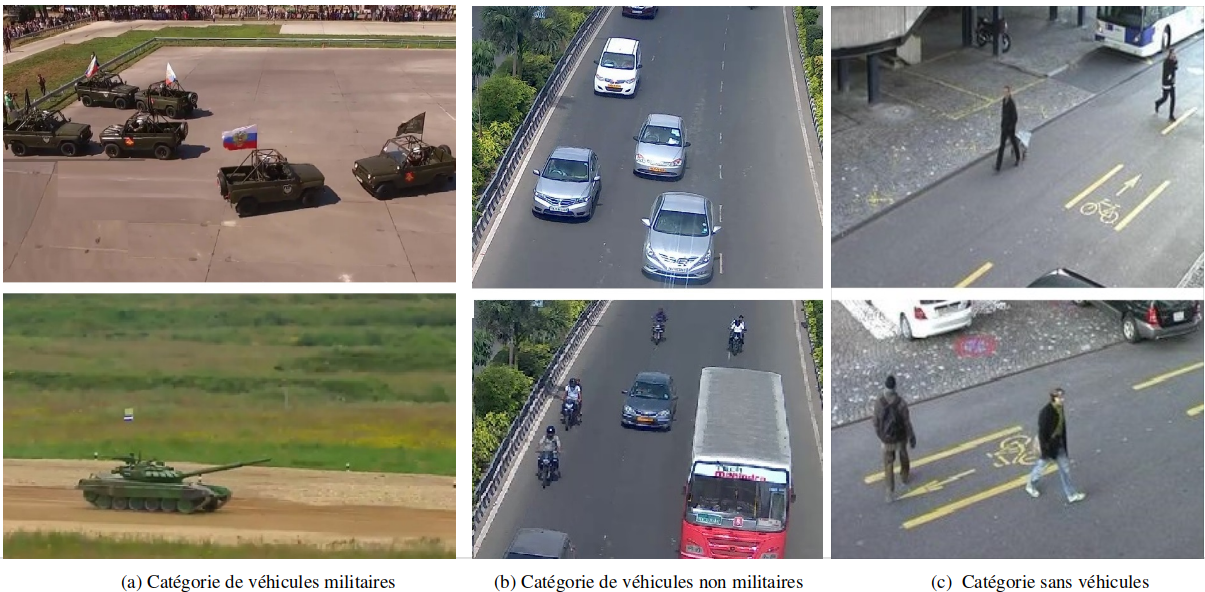
\includegraphics[width=\textwidth]{./images/category-images.png}
    \caption{Quelques catégories d'images \cite[p.~5]{kamran2020}.}
    \label{fig:comparaison_vehicles}
\end{figure}


\section{Détection de Véhicules Militaires}

\subsection{Enjeux et Défis Spécifiques}

La détection de véhicules militaires dans les images aériennes pose des défis particuliers qui ne sont pas rencontrés dans la détection de véhicules civils. Ces défis incluent le camouflage actif, la dissimulation dans des environnements naturels complexes, et la variabilité des configurations de véhicules militaires. Contrairement aux véhicules civils, les véhicules militaires peuvent varier considérablement en termes de taille, de forme et de coloration, ce qui complique davantage leur détection \cite{kamran2020}.

En outre, les véhicules militaires sont souvent capturés dans des conditions difficiles, telles que des angles de vue inhabituels (ex. la Figure~\ref{fig:comparaison_vehicles} des images aériennes prises à basse altitude), des environnements à faible luminosité, ou des contextes où les véhicules sont partiellement cachés ou occultés par d'autres objets. Ces scénarios augmentent la difficulté de la détection, nécessitant des algorithmes capables de gérer ces complexités.

\begin{figure}[H]
    \centering
    \begin{subfigure}[b]{0.45\textwidth}
        \centering
        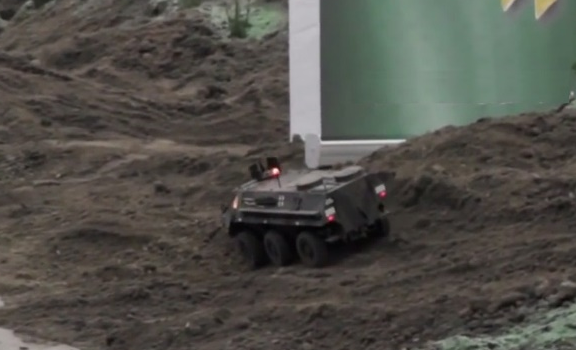
\includegraphics[width=\textwidth]{./images/1-military-vehicul.png}
        \caption{}
    \end{subfigure}
    \hfill
    \begin{subfigure}[b]{0.45\textwidth}
        \centering
        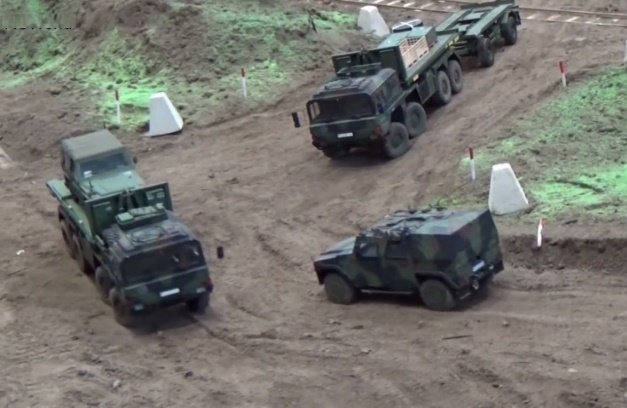
\includegraphics[width=\textwidth]{./images/1-military-vehicul-2.png}
        \caption{}
    \end{subfigure}
    \caption{Images aériennes à basse altitude de véhicules réels \cite[p.~2]{kamran2020}.}
    \label{fig:comparaison_vehicles}
\end{figure}


\subsection{Approches Modernes pour la Détection des Véhicules Militaires}

Les approches modernes pour la détection des véhicules militaires utilisent principalement des techniques de deep learning, avec un accent sur les réseaux de neurones convolutifs (CNN). Quatre architectures principales sont souvent utilisées pour cette tâche : \textbf{Faster R-CNN}, \textbf{YOLOv3}, \textbf{R-FCN} (Region-based Fully Convolutional Networks), et \textbf{SSD} (Single Shot MultiBox Detector). Ces architectures ont montré leur efficacité pour détecter et classifier les véhicules militaires, même dans des environnements complexes et encombrés \cite{kamran2020, gupta2021}.

Parmi ces architectures, Faster R-CNN a démontré une supériorité dans plusieurs études en raison de sa capacité à générer rapidement des propositions de régions et à classifier les objets avec une grande précision. Cependant, pour des véhicules de petite taille ou dans des contextes de faible contraste, des ajustements spécifiques des hyperparamètres et des techniques de data augmentation sont souvent nécessaires pour améliorer les performances des modèles \cite{gupta2021}.

YOLOv3, de son côté, est favorisé pour les applications nécessitant une détection rapide et est capable de traiter des images en temps réel, ce qui est crucial dans des environnements où la rapidité d'intervention est primordiale. Bien que YOLOv3 soit légèrement moins précis que Faster R-CNN pour les objets de petite taille, il offre un bon compromis entre vitesse et précision dans des scénarios militaires \cite{gupta2021}.

L'utilisation de \textbf{datasets spécialisés} est également cruciale. Par exemple, Kamran et al. \cite{kamran2020} ont développé un dataset spécifique pour la détection de véhicules militaires à partir d'images aériennes prises à basse altitude. Ce dataset combine des images réelles et des images synthétiques, permettant ainsi de pallier le manque de données réelles disponibles pour l'entraînement des modèles.

Enfin, les techniques de \textbf{génération de données synthétiques}, comme celles basées sur les GANs (Generative Adversarial Networks), sont de plus en plus utilisées pour enrichir les datasets et améliorer la robustesse des modèles de détection face à la variabilité des conditions d'acquisition des images \cite{spie2020}.

\section{Étude Comparative des Approches}

\subsection{Valeur des Modèles}

Les articles analysés mettent en évidence l'efficacité des modèles de deep learning, en particulier des réseaux de neurones convolutifs (CNN), dans la détection de véhicules militaires. Les études de Kamran et al. \cite{kamran2020} et de Gupta et al. \cite{gupta2021} démontrent que les modèles comme YOLO et Faster R-CNN surpassent largement les méthodes traditionnelles en termes de précision et de rapidité de détection.

Cependant, une comparaison plus détaillée révèle que chaque modèle a ses avantages et ses limitations. Par exemple, \textbf{YOLOv3} est rapide et adapté aux applications en temps réel, mais peut manquer de précision pour les objets de petite taille ou en partie occultés. À l'inverse, \textbf{Faster R-CNN} offre une meilleure précision, mais au prix d'une complexité computationnelle accrue, ce qui le rend moins adapté aux environnements où les ressources sont limitées.

\subsection{Qualité des Données et Entraînement des Modèles}

L'efficacité des modèles de deep learning dépend fortement de la qualité et de la quantité des données utilisées pour leur entraînement. Kamran et al. \cite{kamran2020} soulignent l'importance de disposer de datasets spécialisés, comprenant à la fois des images réelles et synthétiques, pour pallier le manque de données disponibles. Dans le même temps, Gupta et al. \cite{gupta2021} montrent que l'utilisation de techniques de data augmentation est importante pour améliorer la robustesse des modèles face aux variations des conditions d'acquisition des images.

La génération de données synthétiques, notamment via des GANs, est également discutée comme une solution viable pour enrichir les datasets et permettre aux modèles de mieux généraliser. Cependant, cette approche introduit de nouveaux défis, notamment en termes de validation des modèles sur des données réelles.

\subsection{Modèles Utilisés et Performances}

Les performances des différents modèles sont évaluées en fonction de critères tels que la précision de la détection, le taux de faux positifs, et la robustesse face aux variations d'éclairage et de perspective. L'étude de Dijk et al. \cite{spie2020} compare les performances de plusieurs modèles sur des images à longue distance, montrant que les modèles comme \textbf{R-FCN} peuvent offrir un bon compromis entre précision et vitesse dans des environnements complexes.

Néanmoins, la comparaison entre les modèles met également en lumière le besoin d'optimiser les hyperparamètres pour chaque contexte spécifique. Par exemple, l'ajustement des seuils de détection et l'utilisation de techniques de régularisation sont souvent nécessaires pour améliorer les performances dans des conditions de faible visibilité.

\begin{table}[H]
    \centering
    \begin{tabularx}{\textwidth}{|p{3.1cm}|p{2.1cm}|p{1.1cm}|p{2.2cm}|X|c|}
        \hline
        \textbf{Étude}                  & \textbf{Modèle} & \textbf{mAP (\%)} & \textbf{Temps d'inférence (ms)} & \textbf{Données}                & \textbf{Classes} \\ \hline
        Kamran et al. \cite{kamran2020} & Faster R-CNN    & 78                & 220                             & 15 086 (vehicules et personnes) & 3                \\ \hline
        Kamran et al. \cite{kamran2020} & SSD             & 72                & 165                             & 15 086 (vehicules et personnes) & 3                \\ \hline
        Gupta et al. \cite{gupta2021}   & YOLOv3          & 82                & 180                             & 6 772  (vehicules)              & 5                \\ \hline
        Gupta et al. \cite{gupta2021}   & SSD             & 75                & 160                             & 6 772  (vehicules)              & 5                \\ \hline
        Dijk et al. \cite{spie2020}     & CNN             & 55                & 250                             & 7 920  (vehicules)              & 7                \\ \hline
    \end{tabularx}
    \caption{Comparaison des performances des modèles}
    \label{tab:comparaison}
\end{table}

\subsection{Paramètres de Configuration des Modèles}

Les performances des modèles de deep learning dépendent fortement des paramètres de configuration utilisés pendant l'entraînement. Dans cette section, nous comparons les principaux paramètres de configuration pour les modèles étudiés dans les différents articles.

\begin{table}[H]
    \centering
    \begin{tabularx}{\textwidth}{|p{3cm}|p{2cm}|p{2cm}|p{2cm}|p{3cm}|p{2cm}|}
        \hline
        \textbf{Étude}                  & \textbf{Modèle} & \textbf{Taux d'apprentissage} & \textbf{Taille du batch} & \textbf{Nombre d'époques} & \textbf{Taille d'image (px)} \\ \hline
        Kamran et al. \cite{kamran2020} & Faster R-CNN    & 0.001                         & 16                       & 50                        & 600x600                      \\ \hline
        Kamran et al. \cite{kamran2020} & SSD             & 0.002                         & 32                       & 100                       & 300x300                      \\ \hline
        Gupta et al. \cite{gupta2021}   & YOLOv3          & 0.0001                        & 32                       & 70                        & 416x416                      \\ \hline
        Gupta et al. \cite{gupta2021}   & SSD             & 0.002                         & 24                       & 100                       & 300x300                      \\ \hline
        Dijk et al. \cite{spie2020}     & CNN             & 0.0005                        & 24                       & 80                        & 512x512                      \\ \hline
    \end{tabularx}
    \caption{Comparaison des paramètres de configuration des modèles}
    \label{tab:parametres}
\end{table}

Les paramètres de configuration ci-dessus montrent les choix effectués par les auteurs pour optimiser les performances des modèles dans des contextes spécifiques. Par exemple, la taille du batch et le taux d'apprentissage sont importants pour la stabilité et la convergence du modèle. Dans l'étude de Kamran et al., un taux d'apprentissage plus élevé a été utilisé pour SSD, ce qui a permis d'accélérer l'entraînement, bien que cela puisse parfois mener à une instabilité si non contrôlé par un ajustement fin des hyperparamètres. En revanche, Gupta et al. ont opté pour un taux d'apprentissage plus faible pour YOLOv3, privilégiant une convergence plus lente mais plus stable, ce qui est souvent nécessaire pour des architectures complexes comme YOLOv3.

Cette comparaison met en évidence l'importance d'ajuster les paramètres en fonction des spécificités du modèle et du contexte opérationnel, afin de maximiser les performances tout en minimisant les risques d'overfitting ou de sous-apprentissage.

\section{Synthèse}

L'analyse des articles révèle plusieurs défis techniques associés à la détection de véhicules militaires. Parmi eux, la gestion des données limitées et leur qualité, l'optimisation des modèles pour des environnements variés, et la réduction des biais introduits par les datasets sont les plus critiques.

Un point clé soulevé par les études est la nécessité d'une approche équilibrée entre précision et efficacité computationnelle. Bien que des modèles plus complexes comme \textit{YOLOv3} offrent des performances supérieures, leur application en temps réel dans des environnements militaires reste limitée par les ressources disponibles. Par conséquent, des compromis sont souvent nécessaires en fonction des exigences spécifiques de la mission.

Les défis spécifiques de la détection de véhicules militaires nécessitent l'utilisation de techniques avancées de deep learning et de datasets spécialisés. Les progrès récents dans ce domaine, combinés à l'utilisation de données synthétiques et de méthodes de data augmentation, offrent des perspectives prometteuses pour améliorer la précision et la robustesse des systèmes de détection dans des contextes militaires complexes.
